\chapter{Guía de instalación}
\label{chap::instalacion}

\section{Requisitos previos}

Para poder ejecutar BreakBrain el primer paso es instalar (si no se encuentran en nuestro sistema) el entorno de ejecución NodeJS y el \acf{SGBD} MongoDB.

\subsection{NodeJS}

La instalación de NodeJS es realmente sencilla. En la web oficial ({\tt http://nodejs.org}) hay disponibles para descarga multitud de instaladores para diferentes sistemas operativos. Encuentre el adecuado para su sistema y siga los pasos de la instalación.

Alternativamente, y gracias a que NodeJS es software libre, es posible descargar el código fuente y compilarlo de forma manual. Por último, en caso de que nuestro sistema sea GNU/Linux, es posible simplificar al máximo la tarea mediante la utilización de un gestor de paquetes; por ejemplo, en el caso de Ubuntu:

\begin{verbatim}
# apt-get install nodejs  
\end{verbatim}

Una vez instalado NodeJS, desde un intérprete de comandos será posible comprobar que todo ha ido bien, por ejemplo viendo qué versión del binario de NodeJS está disponible en el PATH:

\begin{verbatim}
# node -v
v0.8.5
\end{verbatim}

\subsection{MongoDB}

Una vez que NodeJS se encuentre correctamente instalado en nuestro sistema, el siguiente paso es instalar el \acs{SGBD}.

Al igual que en el caso anterior, la tarea es realmente sencilla siguiendo los pasos de la documentación oficial de MongoDB y usando alguno de los instaladores disponibles en

\begin{verbatim}
http://www.mongodb.org/
\end{verbatim}

Como siempre, si disponemos de GNU/Linux las cosas son aún más sencillas, gracias a los gestores de paquetes. En el caso de Ubuntu:

\begin{verbatim}
# apt-get install mongodb
\end{verbatim}

Una vez instalado, es posible comprobar que el binario se encuentra en el PATH del sistema utilizando un intérprete de comandos para comprobar qué versión se encuentra instalada:

\begin{verbatim}
$ mongo -v
MongoDB shell version: 2.2.3
\end{verbatim}

\section{Instalación de BreakBrain}

Una vez que NodeJS y MongoDB se encuentran perfectamente instalados en el sistema, se estará en disposición de instalar y ejecutar BreakBrain. Para ello se deben seguir los siguientes pasos:

\begin{enumerate}
\item Descargar el código fuente del repositorio oficial ({\tt https://github.com/sgmonda/breakbrain}). Si se dispone de GIT instalado, se puede ejecutar el siguiente comando:

\begin{verbatim}
$ git clone https://github.com/sgmonda/breakbrain
\end{verbatim}

En caso contrario bastará con descargar el siguiente ZIP y descomprimirlo a mano:

\begin{verbatim}
https://github.com/sgmonda/breakbrain/archive/master.zip
\end{verbatim}

\item Abrir un intérprete de comandos y desplazarse al directorio extraído tras la descompresión:

\begin{verbatim}
$ cd breakbrain
\end{verbatim}

\item Instalar las dependencias de BreakBrain, utilizando el gestor de paquetes NPM:
\begin{verbatim}
$ npm install
\end{verbatim}

\item Si todo ha ido bien, ejecutar BreakBrain ahora es realmente sencillo:
\begin{verbatim}
$ node server.js
Tue, 30 Jul 2013 22:48:45 (GMT) :: DATABASE: Connecting to MongoDB...
Tue, 30 Jul 2013 22:48:46 (GMT) :: DATABASE: Connected and authent...
Tue, 30 Jul 2013 22:48:46 (GMT) :: EMAIL-MODULE: Email subsystem r...
Tue, 30 Jul 2013 22:48:46 (GMT) :: GAMES-MODULE: Loading games ser...
Tue, 30 Jul 2013 22:48:46 (GMT) :: WEB SERVER: running on port 206...
Tue, 30 Jul 2013 22:48:46 (GMT) :: GAMES-MODULE: Loading game "Un ...
Tue, 30 Jul 2013 22:48:47 (GMT) :: WEBSOCKETS SERVER: running on p...
Tue, 30 Jul 2013 22:48:47 (GMT) :: MAIN SERVER: The whole server i...
\end{verbatim}
Para ejecutar en modo {\it test}, basta con añadir el flag \verb|--test|:
\begin{verbatim}
node server.js --test
\end{verbatim}

\item En este punto ya es posible utilizar un navegador web para acceder a la copia local de BreakBrain en ejecución, accediendo a {\tt http://localhost:20661}. La página de login se mostrará como en la figura \ref{fig::login}.

\begin{figure}[H]
  \begin{center}
    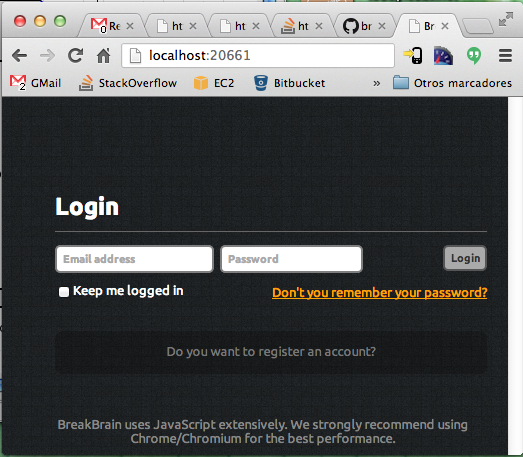
\includegraphics[width=0.8\textwidth]{images/breakbrain-login.png}
    \caption{Página de autenticación de BreakBrain}
    \label{fig::login}
  \end{center}
\end{figure}

\end{enumerate}
